%%%%%%%%%%%%%%%%%%%% author.tex %%%%%%%%%%%%%%%%%%%%%%%%%%%%%%%%%%%
%
% This is the chapter for Reverse Engineering from Natural Language Requirements
%
% It is based on the  sample root file for author's "contribution" to a contributed volume
% 
%
%%%%%%%%%%%%%%%% Springer %%%%%%%%%%%%%%%%%%%%%%%%%%%%%%%%%%


% RECOMMENDED PACKAGES%%%%%%%%%%%%%%%%%%%%%%%%%%%%%%%%%%%%%%%%%%%%%%%%%%%
\documentclass[graybox]{svmult}

% choose options for [] as required from the list
% in the Reference Guide

\usepackage{type1cm}        % activate if the above 3 fonts are
                            % not available on your system
%
\usepackage{makeidx}         % allows index generation
\usepackage{graphicx}        % standard LaTeX graphics tool
                             % when including figure files
\usepackage{multicol}        % used for the two-column index
\usepackage[bottom]{footmisc}% places footnotes at page bottom


\usepackage{newtxtext}       % 
\usepackage{newtxmath}       % selects Times Roman as basic font
\usepackage{booktabs} % For formal tables
\usepackage{pgfplots}
\usepackage{amsmath} %for math environment
\usepackage{paralist} % for tighter & inline itemizations 
\usepackage{xcolor}
\usepackage{multirow} % for tables
\usepackage[toc,page,title,titletoc,header]{appendix} % for appendix
\usepackage{setspace} %for row spacing
\usepackage{wasysym} % for special symbols, as used in the eval table
\usepackage{mdframed}
\usepackage{tikz}
\usepackage[justification=centering]{caption}
\usepackage{ulem} %for underlining
% see the list of further useful packages
% in the Reference Guide

%% Macros
\newcommand{\reftodo}[1]{{\color{red} [REF, #1]}}
\newcommand{\todo}[1]{{\color{red} [#1]}}
\newcommand{\myparagraph}[1]{\noindent\emph{\textbf{#1}}}
\newcommand{\revision}[1]{{\color{blue}#1}}

% define colors
\definecolor{shadecolor}{rgb}{0.92,0.92,0.92}

% define style for the gray boxes
\mdfdefinestyle{mystyle}{
backgroundcolor=shadecolor, 
linecolor=shadecolor
}

% OWN PACKAGES%%%%%%%%%%%%%%%%%%%%%%%%%%%%%%%%%%%%%%%%%%%%%%%%%%%
\usepackage{url}

%%%%%% graphics path and files %%%%%%%%
\graphicspath{{./figs/}}
\DeclareGraphicsExtensions{.eps,.pdf,.bmp,.png,.jpg, .jpeg}

\makeindex             % used for the subject index
                       % please use the style svind.ist with
                       % your makeindex program

%%%%%%%%%%%%%%%%%%%%%%%%%%%%%%%%%%%%%%%%%%%%%%%%%%%%%%%%%%%%%%%%%%%%%%%%%%%%%%%%%%%%%%%%%

\begin{document}

\title*{Feature \& Variability Extraction From Natural Language Requirements}
% Use \titlerunning{Short Title} for an abbreviated version of
% your contribution title if the original one is too long
\author{Sandro Schulze and Yang Li}
% Use \authorrunning{Short Title} for an abbreviated version of
% your contribution title if the original one is too long
\institute{Sandro Schulze 
\at Otto-von-Guericke Universit\"at Magdeburg, Faculty of Computer Science, Universit\"atsplatz 2, 39106 Magdeburg, 
\email{\url{sanschul@iti.cs.uni-magdeburg.de}}
\and Yang Li
\at Otto-von-Guericke Universit\"at Magdeburg, Faculty of Computer Science, Universit\"atsplatz 2, 39106 Magdeburg, 
\email{\url{yang.li@ovgu.de}}
}
%
% Use the package "url.sty" to avoid
% problems with special characters
% used in your e-mail or web address
%
\maketitle

%\abstract*{Each chapter should be preceded by an abstract (no more than 200 words) that summarizes the content. The abstract will appear \textit{online} at \url{www.SpringerLink.com} and be available with unrestricted access. This allows unregistered users to read the abstract as a teaser for the complete chapter.
%Please use the 'starred' version of the \texttt{abstract} command for typesetting the text of the online abstracts (cf. source file of this chapter template \texttt{abstract}) and include them with the source files of your manuscript. Use the plain \texttt{abstract} command if the abstract is also to appear in the printed version of the book.}
\renewcommand{\abstract}[1]{\textbf{Abstract.} #1}
\abstract{Requirements or requirement specifications are usually the very first artifact that is created when starting a software project. 
It results from intensive discussions with customers about all facets of the software system to be developed, mostly in form of plain text. 
Hence, if properly done, requirement specifications reflect on all features of a software system as well as how these features depend on each other. 
Consequently, requirements are a valuable source for extracting variability to support systematic reuse in variant-rich software systems.
We research on techniques that employ syntactical as well as semantical information from such textual requirements in order to 
\begin{inparaenum}[(1)]
\item \textit{extract features} and map requirements to them, and
\item \textit{extract variability} to understand how features are related to each other, and thus, which variants can be possibly created.
\end{inparaenum}
}

\section{Introduction}
\label{sec:intro}
\index{Intro}

Software reuse has been proposed a long time ago as a pivotal aspect of software maintenance and evolution.
While lots of concepts have been proposed for reuse in-the-small (e.g., classes, inheritance, higher-order functions), developing systems for reuse over time and in order to support diverse customer requirements is the grand challenge of today.
Most notably, it is hard to reason about reusable parts (i.e., features) from the beginning (i.e., during requirements analysis) as it is impossible to foresee, which parts should be reused and how should they be modularized for future requirements. Moreover, there is usually no time to perform an in-depth domain analysis that would be necessary for such reasoning.

Think about the following (even though hypothetical) scenario: 
You are running a software company that is working in an increasingly important domain with competitors all over the world.
You are lucky enough to get an offer for developing a software system that would be amazingly important for your business, but you need to be fast enough as your competitors picked up your trail. 
Hence, it all breaks down to the following decision:
\begin{itemize}
    \item[\textbf{Alt1}] Just get started with the project, achieving the goal with incremental refinement and extensions and continuous prototyping, or
    \item[\textbf{Alt2}] Start with high efforts in discussing and eliciting the requirements with the customer, and thereupon, coming up with a proper \textit{software requirements specification (SRS)} as a basis for any further project activity (no matter which type of project management is applied)?
\end{itemize}

Which alternative would you choose?
Obviously, it is tempting to go with \textit{Alt1}, as it promises to deliver a first product relatively fast that can be shown to the customer, and thus, convince her to stay with your company.
However, what if your first prototype is far away from what the customer wants? What if crucial features are not even close to be planned and realized? What if future customer's requirements are diverging or even conflicting with your initial system?

The take away message from this short story is that requirements engineering (and its results) are one of the most crucial yet underestimated parts of the software engineering process since they capture all of the features that should be developed for a particular system.
Of course, this information is not for free: the process of collecting and eliciting requirements is usually a tedious and long-lasting activity, involving many stakeholders, such as customers, managers, developers, and encompassing a series of workshops and interviews.
At the end, the resulting document is a \textit{software requirements specification (SRS)} that constitutes a comprehensive description of any characteristic of the software system that should be developed~\cite{IEEE98}.
As such, it is a valuable source of information to reason about the system, its features and how they are related.

However, an SRS document also comes with some specialities that pose challenges on the analysis of such a document.
First of all, requirements are \textit{textual} documents mostly written in \textit{natural language} with only some basic structure among them. 
Second, compared to other artifacts such as code or models, requirements are rather informal with at most following a certain template or boilerplate~\cite{IEEE98}.
However, they barely follow any strict rules regarding their syntax or composition; in worst case, it is just plain text.
Consequently, analyzing such requirements with the aim of information retrieval is a non-trivial task, as it requires both, syntactic as well as semantic analysis techniques.

Nevertheless, the advantages of requirements for feature \& variability extraction outweigh their shortcomings; if properly maintained, an SRS encompasses all functional and non-functional properties of a system.
Moreover, traceability links to other artifacts in later development stages are usually maintained, and thus, allow for a mapping of such artifacts to their corresponding requirements.
Hence, any information about features that we extract from requirements can be propagated throughout all later development phases.
In particular, we are interested in two different application scenarios for extracting features \& variability from requirements:
\begin{itemize}
    \item[(A)] 
    Software systems that initially start as single program, but over time, features are added that also allow for creating different instances of this system. However, the information about what can be/should be combined and what better not to put into a common program has never been explicated, and thus, needs to be recreated.
    \item[(B)] 
    A software system evolves over time to fulfill the requirements for a particular customer or market.
    At some point, a different customer or market should be satisfied. 
    To this end, the original system is copied and from there on, has its own life (i.e,., evolves independently).
    This process is called \textit{clone-and-own}, can be repeated several times, and is a common reuse mechanism in practice~\cite{DubinskyRBDBC13}, resulting in multiple similar, yet related systems that evolve independently.
    However, with this kind of reuse, all information about differences and commonalities among the resulting variants is usually not documented, and thus, this information is lost or at least hidden from any prospective stakeholder.
\end{itemize}

In this chapter, we will have a closer look on techniques that allow to derive valuable information for both of the aforementioned scenarios from SRS documents. In particular, we focus on two main challenges that are of superior interest in this context:
\begin{center}
    \textbf{How can features be identified in natural language requirements?}
\end{center}
Answering this question is imperative, as features constitute the (logical) building blocks of any product line or variant-rich software system.
Without this knowledge, any task that requires reasoning about features -- testing, specifying feature dependencies, exploring feature interactions -- is impossible.

Unfortunately, there is no universal technique that enables this feature extraction task.
However, since requirements are textual and rather informal, the rise of \textit{natural language processing (NLP)}~\cite{IndurkhyaD10} techniques bear a huge potential to support this task.
We will introduce NLP in general in Section~\ref{sec:nlp} and provide details about techniques for feature extraction (using NLP) in Section~\ref{sec:feature}.

\begin{center}
    \textbf{How can variation points between features be identified?}
\end{center}

Even if we know about the features (and their mapping to the artifacts), we still miss information about their \textit{relationships} and \textit{dependencies} among each other.
This is inevitable, for instance, to reason about valid configurations, apply sampling algorithms~\cite{VarshosazATRMS18}, or to analyze inconsistencies among such relations.

However, since requirements do rarely follow a certain scheme, it is a non-trivial and challenge task to identify those parts that indicate a variation point such as an alternative group or, even harder, a cross-tree constraint.
Only few work exists for this task, which we introduce in more detail in Section~\ref{sec:variability}.
% The research on automatically extracting feature and variability information from natural language documents in the SPLs context started at the beginning of 21st century, on account of the considerable progress in \emph{natural language processing (NLP)}. Generally speaking, the advantages of feature extraction are that: a) natural language documents, such as \emph{software requirements specifications (SRS)}, can be regarded as the initial development artifacts which are able to provide more complete variability information than other artifacts and b) usually traceability links to all other artifacts in later development phases, such as source code or test cases, are maintained. Moreover, by extracting variability information from SRS documents, we can exploit these links for mapping of feature and variability information to other artifacts.


% Example bib reference: \cite{VidyaSagarA14}.

\section{Natural Language Processing in a Nutshell}
\label{sec:nlp}
\index{NLP}

Natural language processing (NLP) is indispensable for feature and variability information extraction from NL documents. It supports computers to analyze, interpret and manipulate human language, paving the way for computer's understanding the human communication. In this section, we will briefly introduce how NLP techniques can be generally utilized to enable feature identification and variation points extraction in SPLs. The general process is shown in Figure~\ref{fig:nlp-general}.

\begin{figure}
\centering
\includegraphics[scale=0.55]{fig_nlp2}
\caption{example graphic, showing a general NLP process for variability extraction}
\label{fig:nlp-general}
\end{figure}

First of all, NL documents are pre-processed by implementing tokenization, assigning parts of speech to each word, removing stop words and so on, which is named \textit{Text Pre-processing}. Given a character sequence, tokenization is the task of breaking it up into pieces, such as words, symbols and other elements called tokens, which makes it easy for computers to identify and analyze NL documents. Moreover, these tokens can be tagged with their type of word (e.g., noun, verb, object, etc.) using \textit{Part-Of-Speech} tagging (POS tagging). Lemmatization can be used to transform different forms of a word into the common base form of the word. For example, the semantically related words, "activates", "activated", "activating", all with similar meaning, are converted into the word "activate". Additionally, stop words which usually refer to the most common words in a vocabulary (e.g., "the", "at", "a") are removed in this phase, as they lack any linguistic information. Note that there doesn't exist a single universal list of stop words that can be selected by means of the specific given purpose. An example for tokenization is as follows:

\vspace{2mm}
\begin{mdframed}[style=mystyle]
\noindent Requirement: \\
``When the alarm system is activated, this is indicated by the light of the LED.''\\ \\
\noindent The corresponding tokens obtained after tokenization: \\
``When'', ``the'', ``alarm'', ``system'', ``is'', ``activated'', ``,'', ``this'', ``is'', ``indicated'', ``by'', ``the'', ``light'', ``of'', ``the'', ``LED'', ``.''
\end{mdframed}
\vspace{4mm}

% \definecolor{shadecolor}{rgb}{0.92,0.92,0.92}
% \begin{shaded}
% \begin{itemize}
%     \item [Requirement:] "When the alarm system is activated, this is indicated by the light of the LED."
%     \item [Tokenization:] 'When', 'the', 'alarm', 'system', 'is', 'activated', ',', 'this', 'is', 'indicated', 'by', 'the', 'light', 'of', 'the', 'LED', '.'
% \end{itemize}
% \end{shaded}

Second, some \textit{Term weighting} techniques are typically used to assess the importance of terms in NL documents usually based on the numerical statistics, such as, computing the frequency of their occurrence in different NL documents. Term Frequency-Inverse Document Frequency (TF-IDF) and C/NC value are two commonly used techniques. 
Generally speaking, TF-IDF relies on the term frequency in a given document and inverse document frequency relies on a collection as a whole, in which the term is considered significant if it appears frequently in a document, but infrequently in other documents. In contrast, C/NC value is a more sophisticated statistical measure which combines linguistic and statistical information~\cite{FrantziAM00}. 

Third, \textit{Semantic Analysis} is optionally applied to achieve the semantic information of the NL documents. Several techniques, such as, Vector Space Model (VSM) and Latent Semantic Analysis (LSA) are widely used to conduct a semantic analysis. More precisely, semantic analysis in this context mostly refers to the distributional semantics research field that analyzes the semantic similarities between linguistic items in terms of the corresponding word vector similarity, while the vector representation is calculated and modelled by words distributional properties in NL documents. Moreover, the cosine value between the vectors are typically used to measure the similarity called cosine similarity.

Finally, after the  general NLP process, a \textit{post-processing} step is indispensable to further analyze the processed NL documents with specific focus on identifying features and extracting variation points. Certainly, various techniques regarding information retrieval and machine learning can be used in this step, such as, Clustering Approaches and Association Rule Mining. Cluster approaches are adopted to group similar features with a feature being a cluster of tight-related requirements. Association rule mining is used to discover affinities among features across products and to augment and enrich the initial product profile. In addition, there are also some rule-based methods in terms of the transformed data by NLP. 

After post-processing, various outputs can be obtained depending on the goal of the analysis and further usage, such as, a feature list, some variation points or an entire feature model. 
Note that the NLP techniques that are appicable in this research area are not limited to aforementioned methods. Moreover, advances in NLP, information retrieval, or deep learning promote the development of feature and variability extraction from NL documents in SPLs.

\section{Feature Extraction}
\label{sec:feature}
\index{Feature}
% 1. feature
%   similarity-based method 
% 2. feature terms (i.e., feature naming)
% 3. traceability link between different artifacts


A feature is the initial and smallest artifact in a feature model. While diverse approaches have been utilized for extracting features from NL documents, we introduce the three most commonly used methods, that is, similarity-based, graph-based, and term-based feature extraction.

\subsection{Similarity-Based Feature Extraction}
% 1. semantic model
% Traditional Distributional Semantic Models
% 2. similarity metric
% 3. clustering

similarity-based feature extraction is the most popular method.
Here, the similarity information among words and sentences is an indispensable property that can be analyzed and utilized for feature extraction from NL documents.
In order to achieve the similarity value for each pair of words, sentences or requirements, various similarity measures can be employed, such as, string-based, corpus-based and knowledge-based similarity~\cite{GomaaFA13}. In the context of feature extraction from requirements, the most commonly used similarity measures are \textit{corpus-based} and \textit{knowledge-based} similarity~\cite{LiSS17}. The reason is that the similarity value for each pair of requirements highly depends on the semantic information of the requirements, while string-based similarity measure lack the capability of achieving accurate semantic information.

\begin{figure}
\centering
\includegraphics[scale=0.4]{figs/similar_feature.png}
\caption{A general process for similarity-based feature extraction}
\label{fig:similar_feature}
\end{figure}

In Fig. \ref{fig:similar_feature}, we show the general work flow regarding similarity-based feature extraction. Besides tokenization , lemmatization, and removing stop words, a POS filter is commonly used during pre-processing in order to select the most meaningful words, such as nouns, adjectives, and verbs. After the pre-processing step, different similarity measures can be applied to achieve the similarity information encompassing the similarity values and a similarity matrix regarding the words, sentences, or requirements. Then, the obtained similarity information is further analyzed using different approaches, such as clustering algorithms or even manual analysis. Certainly, \textit{clustering algorithms} are the most commonly used methods to automate the analysis, where similar information (e.g., words, sentences, requirements) are grouped in terms of the \textit{similarity matrix} of the requirements. Finally, the features can be identified based on the resulting clusters (i.e., groups of similar information), taking different rules or heuristics into account.

\subsubsection{Similarity Measures}
\textit{\textbf{Corpus-based similarity.}}
The semantic similarity of words, sentences or texts is obtained in terms of a numeric representation learned from the semantic information of a large text collection, called corpus-based similarity. In our case, the corpora can be any text collection regarding the products or systems in a specific domain, such as SRS. There are two kinds of corpus-based similarity measures commonly used to achieve the similarity: traditional distributional semantic models (DSMs) and neural word embedding.

\myparagraph{Traditional DSMs} can be considered as count models, since they operate on co-occurrence matrices to initialize the vector representation of words, such as counting co-occurrences of words appearing in a specific corpus. VSM and LSA are traditional DSMs that are commonly applied in the research area for feature extraction from requirements \cite{KumakiTWF12,AlvesSBRSRPR08,WestonCR09}.

The basic idea behind VSM is to transform the text content to vector operations in vector space. To this end, spatial similarity (i.e., the similarity of vectors) is used to express semantic similarity of texts, which is intuitive and easy to understand~\cite{SaltonWY75}. When a document is represented as a vector, the similarity between documents can be measured by calculating the similarity between the vectors. The most commonly used measure of similarity in text processing is the cosine distance. Next, we briefly introduce how to obtain the vector representation of requirements. Given a set of requirements $R$ and a dictionary $D$, a requirement is represented as the bag of its words (i.e., the bag-of-words model), and then a value is calculated for each word according to the TF-IDF.
Given the size of dictionary $D$ being $m$, the requirement is converted into an $m$-dimensional vector. If a word in the dictionary does not appear in a particular requirement, the corresponding element of the word in the vector is 0. If a word appears in the requirement, the corresponding element value of the word in the vector is the TF-IDF value of the word. This way, the requirement is represented as a vector, which forms the foundation the vector space model.To put it differently, the vector space model does not catch the relationship between terms, but rather assumes that terms are independent of each other.

LSA also treats the text as a document-term matrix and calculates the similarity between documents by vectors (e.g., based on the angle), which is the same as VSM. The difference is that LSA assumes that some latent structures exist in word usage to express a topic, but these latent structures may be partially obscured by the variety of word selections. Hence, LSA utilizes singular value decomposition (SVD) to the document-term matrix and takes the first $k$ largest singular values and corresponding singular vectors to form a new matrix~\cite{Dumais04}. The new matrix reduces the ambiguity of the semantic relationship between terms and text, which is beneficial to figure out the meaning of text.

\myparagraph{Neural word embedding} is a neural-network-based natural language processing architecture which can be seen as prediction models, since the vector representations of words or texts can be gained from a pre-trained language model trained on a large text collections by using neural network technique. To this end, also various techniques exist to achieve accurate neural word embedding models, such as word2vec \cite{MikolovSCCD13}, GloVe \cite{PenningtonSM14} and FastText \cite{BojanowskiGJM16}.

Word2vec applies a two-layer neural network to train a large-scale corpus, which results in a vector space where the words in the corpus are transformed into vector representation in the vector space. Its basic idea is that two words with similar context (i.e., surrounding words) should have similar word vectors. According to the difference of using the context, word2vec provides two methods to achieve the representations of languages: the Continuous Bag-of-Words (CBOW) and Skip-gram models. As shown in Figure~\ref{fig:word2vec}, the CBOW predicts the target word based on the context, while based on the word, Skip-gram predicts the target context.

\begin{figure}
\centering
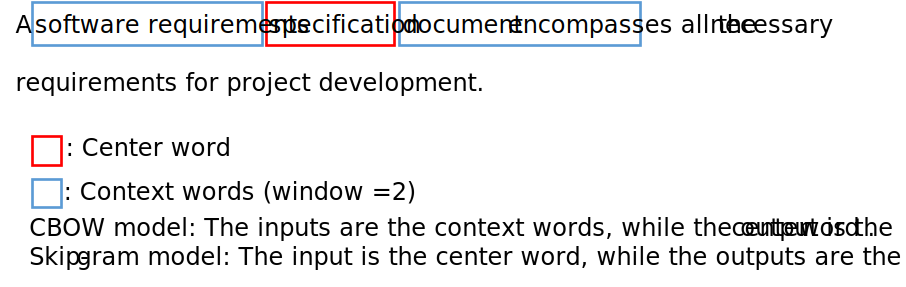
\includegraphics[scale=0.49]{figs/word2vec.pdf}
\caption{An example for sketching the CBOW and Skip-gram models}
\label{fig:word2vec}
\end{figure}

Word2vec is trained on a local corpus, and its text characteristic extraction is based on sliding windows, while GloVe's sliding windows are used to build a co-occurance matrix, which is based on a global corpus. As a consequence, GloVe needs to count the co-occurrence probability in advance. FastText treats each word as a bag of n-grams rather than the word itself. For example, the n-gram representation of word ``apple'' for $n=3$ is ``<ap'', ``app'', ``ppl'', ``ple'', ``le>'' with boundary symbols ``<'' and ``>''. As a result, we can use these tri-grams to represent the word ``apple''. Moreover, the sum of these five tri-grams vectors can be used to represent the word vector of ``apple''. Additionally, Fasttext can learn the vector of the character n-grams in a word and sum these vectors to generate the final vector of the word itself, and thus, generate a vector for a word that does not appear in the training corpus.

\textit{\textbf{Knowledge-based similarity.}}
The similarity among words depends on the degree of the words' semantic relatedness drawn from semantic networks or knowledge bases, called knowledge-based similarity \cite{MihalceaCS06}. WordNet as a large knowledge base has been extensively used to achieve the semantic relatedness of words in various research areas. It is a large lexical database of English in which nouns, verbs, adjectives and adverbs are grouped into sets of cognitive synonyms, each expressing a distinct concept \cite{Miller95}. In WordNet, synsets denote the sets of cognitive synonyms, interlinked by means of conceptual-semantic and lexical relations. There exist some approaches that uses WordNet in the process of feature extraction. For example, WordNet can be applied to identify synonyms to group verbs with similar senses~\cite{Wang15,Wang16}, while in research~\cite{ItzikR14,ItzikRBW16}, WordNet is utilized to compute the similarity of two words based on the depth of the two senses in the taxonomy in WordNet ontology. 
Besides achieving the similarity, WordNet is employed to extract the hierarchy of features by taking advantage of the hypernyms and hyponyms of the feature names~\cite{MeftehBB16}.


\subsubsection{Rules \& Heuristics}
The rule-based methods and heuristics are typically used to analyze and process the requirements in order to extract features, taking the different kinds of similarity information into account.

\textit{\textbf{Semantic roles.}} 
In some research \cite{ItzikR14,ReinhartzIW14}, the requirements are further analyzed and processed to extract some predicated semantic roles (e.g., agent, action, object, ect) from each individual requirement based on Semantic Role Labelling (SRL) technique. The similarity of each pair of requirements relies on the weighted average similarity of the predicated semantic roles in the requirements.

The SRL task refers to the predicate of the sentence as the center. 
However, it does not analyze the semantic information contained in the sentence in depth, but only analyzes the relationship between each component (i.e., semantic argument) in the sentence and the predicate (i.e., verb), namely the Predicate-Argument structure. 
Moreover, SRL describes these structural relationships with semantic roles, such as Agent, Patient, Theme, Experiencer, Beneficiary, Instrument, Location, Goal, Source, and so on~\cite{PalmerGK05}.

\textit{\textbf{Clustering algorithms.}}
Commonly used methods to analyze the similarity information automatically are clustering algorithms, such as, K-means, hierarchical clustering and DBSCAN. The indispensable assumption is that, for example, if we assume that several requirements related to similar functionality belong to a particular feature, we can observe that a cluster denotes a feature. 

Moreover, hierarchical clustering algorithms are not only used to extract features from requirements, but can also be applied to achieve the hierarchy of features by inheriting the cluster tree (i.e., a dendrogram), such as in several proposed approaches~\cite{AlvesSBRSRPR08,WestonCR09,ItzikR14,LiSS18}. More precisely, we can cut the tree at a predefined distance to gain features (i.e., clusters) and keep the hierarchy information. For example, in Figure~\ref{fig:hac}, given the distance threshold as 20, we can achieve three concrete features marked as green, red and peacock blue, respectively. According to the cluster tree, we can also infer that there might exist an abstract feature that is the parent feature of the two concrete features marked as red and peacock blue.

\begin{figure}
\centering
\includegraphics[scale=0.4]{figs/hac.pdf}
\caption{The dendrogram in the HAC}
\label{fig:hac}
\end{figure}

\subsection{Graph-Based Feature Extraction}


Graph-based approaches constitute another method for feature extraction. In graph theory, a graph is a network of a set of objects, where some pairs of objects are related with each other in a certain, well-defined way. Generally, we use vertices (i.e., points or nodes) to represent the objects and edges (i.e., lines) to represent the relation between (pairs of) vertices. In other words, a graph is a set of vertices connected with edges, denoted as $G = (V,E)$. 
Moreover, a graph can have further properties such as being \textit{directed/undirected} or a \textit{weighted graph}.
%$In the context of SPLs, a graph $G = (V,E)$ in which vertex $V$ and edge $E$ can be defined as diverse forms. 

 As an example for graph-based extraction approaches, we briefly introduce a technique by Chen et al.\ that uses a weighted, undirected graph for feature extraction~\cite{ChenZZM05}. 
 In particular, they use this graph to illustrate several dedicated relationships between individual requirements. 
 To this end, vertices denote individual requirements, while edges represent the dedicated relationships between pairs of requirements. 
 Moreover, the weight of each edge is used to measure the strength of the relationships between requirements. 
 In particular, they predefined five relationships between requirements in terms of whether the two requirements access or modify the same data, while the weight of each relationship is determined by domain engineers. Since there may exist more than one relationship between two requirements, the weight value of each edge is the sum of the weights of all relationships of the corresponding two requirements.
 
After the graph construction, requirements are clustered by a comparison between the weight values of each edge and a preset threshold value that must be exceeded.
As a result, the finally created cluster constitute the features with the threshold determining the granularity of features.
The rationale behind this technique is that strongly related requirements (by means of data flow) belong to the same feature.
Furthermore, the hierarchy of features is obtained by means of comparing whether a feature is another feature's subset. For example, let us assume that there is a feature $A$ containing three requirements $R1$, $R2$ and $R3$, while feature $B$ comprises $R2$ and $R3$. Then, the described technique identifies feature $A$ as the parent feature of feature $B$, because feature $B$ comprises a subset of the requirements of feature $A$. 
The method mentioned above can be used to initially achieve application feature trees by analyzing the functional requirements of different but similar applications. Afterwards, the application feature trees are merged into a single domain feature tree by the occurrence of features in both application feature trees and domain feature tree. 
Eventually, manual intervention is necessary to refine the results of the application feature trees and domain feature tree.

Moreover, the graph-based method is not only able to identify features, but also capable of extracting variability information (cf. Section \ref{sec:variability}), especially for the application of \textit{directed graph}.

% 1. features are clustered by the weights between two requirements in an undirected graph. \cite{ChenZZM05}

% \textit{\textbf{Directed graph.}}
% 2. Association rule mining. \cite{DavrilDHACH13}

% 3. \cite{AcherCPHVCL12}

\subsection{Feature Term Extraction}
\label{subsec:FTE}
In NL documents, there usually exist some domain specific terms representing the concrete functionality in a system. Hence, it is possible to use the specific term to denote a feature, called \textit{feature term}.
For example, in the requirement below:

% \definecolor{shadecolor}{rgb}{0.92,0.92,0.92}
% \begin{shaded}
% "The \underline{interior monitoring} is deactivated as soon as the \underline{alarm system} is deactivated."
% \end{shaded}
\vspace{2mm}
\begin{mdframed}[style=mystyle]
``The \uline{interior monitoring} is deactivated as soon as the \uline{alarm system} is deactivated.''
\end{mdframed}
\vspace{4mm}

Since the terms, "interior monitoring" and "alarm system", denote the specific functionality of the system, both terms can be considered as feature terms. These feature terms not only constitute possible feature names, but also can be used to detect variability information, taking the syntax of the requirements into consideration. 

Generally, different NLP techniques are capable of extracting feature terms, such as keyword extraction or Named Entity Recognition (NER). In the context of SPLs, \textit{POS pattern} is a common keyword extraction method to identify meaningful terms.
For example, "alarm system" can be identified by a \textit{<noun, noun>} pattern, whereas "interior monitoring" can be identified by a \textit{<adj, noun>} pattern. 
The NER technique is utilized for identifying the named entities of things in NL documents, such as people and organization names, or gene and protein names. In the context of SPLs, a feature term is regarded as a named entity. Since we lack open source pre-trained NER models for feature term extraction, we first of all have to train a NER model by using a labelled dataset. In related work~\cite{BagheriEG12}, there is an example of how the requirements are labeled in the context of NER for feature extraction:

\vspace{2mm}
\begin{mdframed}[style=mystyle]
``A graph is an abstract mathematical representation that is used for exemplifying inter-entity relationships. Graphs can have different types. They can be \uline{directed} or \uline{indirected}; \uline{weighted} or \uline{unweighted}. A graph cannot be both directed and undirected. A graph can either be weighted or unweighted. One of the most desirable operations on a graph is the \uline{search} operation. Graphs can be searched using \uline{depth-first} or \uline{breadth-first} strategies...''
\end{mdframed}
\vspace{4mm}

The underlined terms are labeled as potential features. Moreover, we also need to identify the characteristics\footnote{In machine learning, features are observable or derived properties of a phenomenon in a specific domain. In order to distinguish from the features in the context of SPLs, we utilize \textit{characteristics} to denote features in machine learning.} of these labeled requirements for the learning step, such as, the word level characteristics (e.g., n-gram, lowercase, uppercase, token length, POS)~\cite{NadeauS07}.

\subsection{Evaluation Metric}

In order to properly conduct a quantitative analysis of the results, the measures \textit{precision}, \textit{recall} and \textit{F1 score} are usually used to evaluate the results of the extracted features. The equations for each measure are shown below:

\begin{equation}
Precision = \frac{The\ number\ of\ extracted\ true\ features}{ The\ number\ of\ all\ extracted\ features}
\end{equation}

\begin{equation}
Recall = \frac{The\ number\ of\ extracted\ true\ features}{ The\ number\ of\ features\ in\ ground\ truth}
\end{equation}

\begin{equation}
F1 = 2 \times \frac{Precision \times Recall}{Precision + Recall}
\end{equation}

From the equations above, we can see that if we intend to achieve the quantitative analysis of the results by using precision, recall and F1 score, the ground truth of the features in a particular SPL is indispensable.


\section{Variability Extraction}
\label{sec:variability}
\index{Variability}
While features are the building blocks of the envisioned domain-feature model, we also need to know about their corresponding variability, that is, how and when a feature must (not) be selected for a certain configuration.
Extracting such variability information requires multiple NLP tasks to reveal different relations among features. 
While \textit{heuristics} or \textit{rule-based} methods are predominantly utilized to further analyze the information from the \textit{occurrence} of requirements and terms, \textit{lexical analysis}, \textit{syntactic analysis}, \textit{association rule mining} and \textit{NER} are used to infer the potential variability information from requirements.

\subsection{Optionality}
Several approaches exist to detect the optionality (i.e., mandatory and optional). 
We introduce the three most common methods below.

\textit{\textbf{Occurrence.}} The most popular method is to apply heuristics or pre-defined rules to detect the optionality based on the occurrence of requirements or domain-specific terms in different variants. 
For example, we can simply define the following rule: if a feature has been extracted from some requirements and these requirements are present in all the variants, the feature is mandatory; otherwise, the feature is optional. Although the rules vary depending on the concrete research topic, the foundation of the rules is the distribution of features across different variants, which can be considered as \textit{traceability link} between features and variants.

The general process for establishing such traceability links is as follows:
\begin{enumerate}
    \item If the set of requirements contains the corresponding variants information (i.e., in which variants certain requirements are present), we can directly obtain a mapping between requirements and variants.
    \item After feature extraction, the approach we used is capable of achieve a mapping between features and requirements.
    \item Based on the aforementioned two mappings, we can achieve a traceability link between feature and variants.
    \item Regarding the distribution of features across different variants, we now know whether a variant includes a certain feature or not. Hence, different methods such as heuristics can now be applied to extract the optionality.
\end{enumerate}

It is worth to mention that the two-step mapping approach is kind of a bridge used to connect the features and variants. Generally, such a bridge can be constructed by other mappings as well, such as a mapping between domain-specific terms and variants \cite{FerrariSD13}. 
The underlying idea is that the distribution of different features across different variants can be regarded as a kind of domain knowledge, while we use statistics to quantify this kind of domain knowledge in order to further detect the optionality.

% 1. Occurrence in variants. mandatory and optional is extracted by calculating the occurrence of dedicated attribute \cite{ChenZZM05} or artifacts (requirements \cite{SPLC paper} \cite{WestonCR09} \cite{ItzikR14} , domain-specific terms \cite{FerrariSD13}).  

\textit{\textbf{Lexical analysis.}} Another regularly applied method is to analyze some specific words appearing in the requirements, such as adjectives (e.g., "possible"), model verbs (e.g., "must"), adverbs (e.g., "optionally") and etc.. 
For example, in the requirement below \cite{Sree-KumarPC18}:

% \definecolor{shadecolor}{rgb}{0.92,0.92,0.92}
% \begin{shaded}
% "The \underline{publishing module} \textit{\textbf{can}} be configured using a \underline{custom reports module}." 
% \end{shaded}
\vspace{2mm}
\begin{mdframed}[style=mystyle]
``The \uline{publishing module} \textit{\textbf{can}} be configured using a \uline{custom reports module}.'' 
\end{mdframed}
\vspace{4mm}

The model verb "can" represent a possibility, from which the relationship between the two feature terms, "publishing module" and "custom reports module", are able to be deduced as optional.


% 2. Lexical analysis. The determination of whether a feature is optional, alternative, or or-feature is performed by analyzing the context of its requirements by searching for words denoting these concepts (e.g., "optionally", "alternatively", "at least one of"). \cite{AlvesSBRSRPR08} \cite{Laura's VaMos paper} \cite{AcherCPHVCL12} 
%  \cite{P2 see excel sheet} defined some rules in terms of the occurrence and position of some special words

\textit{\textbf{Association rule mining.}} The optionality can also be detected by identifying associations between features based on association rule mining, one of the popular data mining techniques. For example, Davril et al. proposed to use an implication graph, a \textit{directed graph}, where vertex denotes a feature and edge denotes the confidence between the two connected features to determine whether a feature is mandatory or not \cite{DavrilDHACH13}.

% 3. Association rule mining. \cite{DavrilDHACH13}


% 4. \cite{HamzaW15} mandatory and optional features are identified by heuristics (actor, action, and object)

\subsection{Group Constraints}
The methods for group constraints (e.g., Or-Group and XOR-Group) extraction are predominantly related to the techniques used for optionality extraction.

\textit{\textbf{Occurrence.}} In previous work of Itzik et al. \cite{ItzikR14}, feature models are generated by grouping similar requirements based on a hierarchical clustering algorithm, including some abstract and concrete features. 
Moreover, in their model, each concrete feature denotes an individual functional requirement. Moreover, two rules are pre-defined for group constraints extraction:

% \definecolor{shadecolor}{rgb}{0.92,0.92,0.92}
% \begin{shaded}
% \begin{itemize}
%     \item [1.] If at least two requirements that are grouped under the same parent node appear in the same input document, then the corresponding requirements are \textit{OR-grouped}.
%     \item [2.] If requirements originating from different input files are grouped under the same parent node, we consider the corresponding requirements as \textit{XOR-grouped}.
% \end{itemize} 
% \end{shaded}

\vspace{2mm}
\begin{mdframed}[style=mystyle]
\begin{itemize}
    \item [1.] If at least two requirements that are grouped under the same parent node appear in the same input document, then the corresponding requirements are \textit{OR-grouped}.
    \item [2.] If requirements originating from different input files are grouped under the same parent node, we consider the corresponding requirements as \textit{XOR-grouped}.
\end{itemize} 
\end{mdframed}
\vspace{4mm}


In the two rules above, the input documents/files can be regarded as variants. 
Moreover, the parent node of the feature model constitutes an abstract feature, while each requirement constitutes a concrete feature. Hence, similarly to extracting optionality, the distribution of features across variants can also be applied to extract the group constraints. 
Note that further rules are defined in abovementioned paper~\cite{LiSS18}.


% 1. Occurrence in variants. \cite{ItzikR14} \cite{SPLC aper}

\textit{\textbf{Lexical analysis.}} For extracting group constraints based on lexical analysis, we also illustrate an example from Sree-Kumar et al.~\cite{Sree-KumarPC18}:
% \definecolor{shadecolor}{rgb}{0.92,0.92,0.92}
% \begin{shaded}
% "We believe that \underline{proof of individuality (POI)} \textit{\textbf{can}} be better solved with \underline{biometrics} than what is currently being proposed in the Ethereum community - \underline{a series of video calls}."
% \end{shaded}

\vspace{2mm}
\begin{mdframed}[style=mystyle]
``We believe that \uline{proof of individuality (POI)} \textit{\textbf{can}} be better solved with \uline{biometrics} than what is currently being proposed in the Ethereum community - \uline{a series of video calls}.''
\end{mdframed}
\vspace{4mm}



We can deduce that there two potential sub-features, "biometrics" and "a series of video calls", belonging to "proof of individuality". In terms of the specific model verb "can", we can deduce that the two sub-features may or may not coexist when the parent feature is configured. Hence, the two sub-features are possibly or-grouped.

% 2. Lexical analysis. The determination of whether a feature is optional, alternative, or or-feature is performed by analyzing the context of its requirements by searching for words denoting these concepts (e.g., "optionally", "alternatively", "at least one of"). \cite{AlvesSBRSRPR08}

\textit{\textbf{Association rule mining.}} As the aforementioned optionality extraction based on implication graphs drawn by association rule mining \cite{DavrilDHACH13}, the or-group relation can also be detected by the vertex (i.e., concrete feature) of an implication graph. If an abstract feature can be comprised of concrete features from the vertices in the implication graph, these concrete features are regarded as or-grouped features.

% 3. Association rule mining. \cite{DavrilDHACH13}
% 4. \cite{AcherCPHVCL12}

\subsection{Cross-Tree Constraints}
\textit{\textbf{Lexical and syntactic analysis.}} Based on the feature term extraction (cf.\,Section~\ref{subsec:FTE}), we can further analyze the lexical and syntactic information of requirements containing feature terms in order to detect the cross-tree constraints between features. 

For lexical analysis, here is an example from Sree-Kumar et al.~\cite{Sree-KumarPC18}.
% \definecolor{shadecolor}{rgb}{0.92,0.92,0.92}
% \begin{shaded}
% "\underline{Headphones} are generally provided for \textit{\textbf{all}} devices with \underline{FM radio} capability."
% \end{shaded}

\vspace{2mm}
\begin{mdframed}[style=mystyle]
``\uline{Headphones} are generally provided for \textit{\textbf{all}} devices with \uline{FM radio} capability.''
\end{mdframed}
\vspace{4mm}

They assume that the predeterminers assists the inference of cross-tree constraints between feature terms. Hence, in the requirement above, the predeterminer "all" is regarded as presenting a require relation between "headphones" and "FM radio".


For usage of syntactic information, we can simply define a rule that there exist potential cross-tree constraints between feature terms in main clause and modifier clause (e.g., temporal or adverbial clause). 
% \definecolor{shadecolor}{rgb}{0.92,0.92,0.92}
% \begin{shaded}
% "When the \underline{alarm system} is activated, this is indicated by the light of the \underline{LED}."
% \end{shaded}

\vspace{2mm}
\begin{mdframed}[style=mystyle]
``When the \uline{alarm system} is activated, this is indicated by the light of the \uline{LED}.''
\end{mdframed}
\vspace{4mm}

In the above example, there is requirement including a temporal clause. Based on the pre-defined rules we can observe that the light of "LED" require the activated "alarm system".

\textit{\textbf{NER.}} WHile we introduced NER as a technique to extract features, it is also possible to apply NER  for detecting cross-tree constraints. 
First of all, if there is no pre-trained NER model, we need to train a NER model by a labelled dataset. In this labelled dataset, the requirements containing specific cross-tree constraints are assigned a dedicated label. An example of labelled requirements \cite{BagheriEG12} is shown below:

% \definecolor{shadecolor}{rgb}{0.92,0.92,0.92}
% \begin{shaded}
% "A graph cannot be both directed and undirected" and "A graph can either be weighted or unweighted" are labelled as \textit{\textbf{ic}}.
% \end{shaded}

\vspace{2mm}
\begin{mdframed}[style=mystyle]
``A graph cannot be both directed and undirected'' and ``A graph can either be weighted or unweighted'' are labelled as \textit{\textbf{ic}}.
\end{mdframed}
\vspace{4mm}

The label \textit{ic} denotes integrity constraints (i.e., cross-tree constraints). The label is just symbol used to indicate that there are potential cross-tree constraints in the requirements.

% 1. NER \cite{BagheriEG12}

% 2. Association rule mining. \cite{DavrilDHACH13}

\subsection{Evaluation Metric}

We can also use the \textit{precision}, \textit{recall} and \textit{F1 score} to conduct the quantitative analysis of the extracted variability information. The equations are shown below:

\begin{equation}
Precision = \frac{The\ number\ of\ extracted\ true\ variation\ points}{ The\ number\ of\ all\ extracted\ variation\ points}
\end{equation}

\begin{equation}
Recall = \frac{The\ number\ of\ extracted\ true\ variation\ points}{ The\ number\ of\ variation\ points\ in\ ground\ truth}
\end{equation}

\begin{equation}
F1 = 2 \times \frac{Precision \times Recall}{Precision + Recall}
\end{equation}

Likewise, the ground truth of the variability information is required in the process of achieving the quantitative analysis.


\section{Related Work}
All the techniques introduced above are used to process natural language requirements documents for extracting features and variability information, which allows for a more efficient way to conduct domain analysis than only depending on manual analysis for processing textual requirements.
In order to understand the general applicability of the techniques for feature and variation points extraction, we categorize related work in terms of the type of \textit{input} documents, the type of \textit{output} and the specific \textit{supposition}. We list the different kinds of inputs, outputs and suppositions in Table~\ref{tab:types_ios}.



\begin{table}[]
\centering
\caption{The types of inputs, outputs, and suppositions}
\label{tab:types_ios}
\begin{tabular}{p{2.2cm}|p{1cm}|p{8cm}}
\toprule
Interests/Goals                         & Types   & Descriptions                                                                                                                                  \\ \midrule

\multirow{2}{*}{Condition} & Con1 & The formal SRS documents are reachable.                                          \\ \cline{2-3} 

        & Con2 & The formal SRS documents are not reachable. \\ \hline
\multirow{5}{*}{Input}       & In1  & Functional requirements with simple and uniform format.                                                                                       \\ \cline{2-3} 
                             & \multirow{2}{*}{In2}  & Requirements specification documents written by different formats.                                                                                          \\ \cline{2-3} 
                             & In3  &  Other informal textual documents.                                                         \\ \cline{2-3} 
                             & \multirow{3}{*}{In4}   & The requirements specification documents (or other informal textual documents) come from different products or applications in a particular domain.                                                                                                               \\ \hline
\multirow{3}{*}{Output}      & Out1 & (list of) Features.                                                                                                                                     \\ \cline{2-3} 
                             & Out2 & Feature model.                                                                                                                                \\ \hline
\multirow{6}{*}{Supposition} & \multirow{2}{*}{Sup1} & A feature as a high-level abstraction of a group of requirements semantically similar to each other.                                          \\ \cline{2-3} 
                             & \multirow{3}{*}{Sup2} & A feature as a high-level abstraction of a group of requirements that are similar not only semantically but also from a specific perspective. \\ \cline{2-3} 
                             & Sup3 & A feature as a term comprised of words or phrases.                                                                                            \\ \bottomrule                             
\end{tabular}
\end{table}


% The types of the inputs:
% \begin{itemize}
% \end{itemize}
% \begin{itemize}
%     \item[In1:] Functional requirements with simple and uniform format;
%     \item[In2:] Requirements documents written by different formats;
%     \item[In3:] Requirements documents from different products or applications in a particular domain;
%     \item[In4:] Other artifacts or documents.
% \end{itemize}
% The types of the outputs:
% \begin{itemize}
%     \item[Out1:] Features;
%     \item[Out2:] Variability information;
%     \item[Out3:] Feature model.
% \end{itemize}
% The types of the suppositions:
% \begin{itemize}
%     \item[Sup1:] A feature as a high-level abstraction of a group of requirements semantically similar to each other;
%     \item[Sup2:] A feature as a high-level abstraction of a group of requirements that are similar not only semantically but also from a specific perspective;
%     \item[Sup3:] A feature as a term comprised of words or phrases.
% \end{itemize}


\noindent\textbf{\textit{Con1, In2 and In4, Out2, Sup1:}}
Dubinsky et al.~\cite{AlvesSBRSRPR08} apply VSM and LSA to achieve similarity matrices of requirements documents with different structures and formats. Subsequently, the similarity matrices are fed into HAC to achieve different initial feature trees. 
Finally, the different initial feature trees are merged into the final feature model by manual analysis. In the evaluation, they apply two different requirements specification documents from a Smart Home case study as input.Moreover, they compare the clustering results  between VSM+HAC and LSA+HAC, reporting the observation that for the small size of the individual requirements, VSM might outperform LSA. However, there is no evaluation regarding the features, variability information, and feature model.
As an alternative approach, Li et al.\,combine BM25+ and word2vec instead of VSM and LSA to obtain the similarity of each pair of requirements~\cite{LiSS18}.

\noindent\textbf{\textit{Con1, In1 or In2, Out2, Sup1:}}
In~\cite{WestonCR09}, LSA and HAC are also applied to cluster similar requirements into features. Afterwards, the features grouped using HAC are directly regarded as mandatory features, resulting in an initial feature tree. The variant features are identified manually with the assistance of the results of variability lexicon and grammatical pattern identifier, thereby obtaining the final feature model.

\noindent\textbf{\textit{Con1, In1 and In4, Out2, Sup2:}} Itzik and Reinhartz-Berger et al. conducted a series of research~\cite{ItzikR14, ItzikRBW16, ReinhartzIW14} on extracting features and analyzing the variability information in terms of behaviors of the software products extracted from functional requirements. They identify behavioral vectors from the requirements, while each behavioral vector contains six semantic roles extracted by semantic role labeling. 
In the next step, the extracted behavioral vectors are classified into different behavioral elements (i.e., initial state, external event, and final state) that are used to denote the initial/final state of a system before/after a behavior occurs, and the corresponding external event triggering the behavior. 
Afterwards, the similarity of the requirements is computed by using Mihalcea, Corley, and Strapparava's (MCS) measure that is based on WordNet. 
Moreover, MCS also takes the behaviors into account when calculating the similarity, for example, assigning different weights for the semantic roles and behavioral elements.
This approach also relies on HAC to obtain the initial feature tree.
Additionally, the variability information, such as optionality and group constraints, is detected by predefined rules which are created by taking into account the occurrence of the individual requirements in the requirements documents from different applications. We can observe that
\begin{inparaenum}[a)]
\item in order to achieve accurate behaviors, the requirements should be well written in a uniform format, especially for the automated extraction; and
\item The input requirements should come from different applications in the same domain. Otherwise, the rules for detecting variation points can not be used.
\end{inparaenum}

\noindent\textbf{\textit{Con1, In1 and In4, Out2, Sup3:}} In~\cite{MeftehBB16}, Mefteh et al. use a dedicated semantic model to process the requirements to achieve the corresponding mapping rules that are able to present each sentence in the requirements in a formal and unique way. By using such mapping rules, information such as the type of sentences, syntax, and semantic roles can be extracted. 
Moreover, they perceive the \textit{terms} identified from the mapping rules and denoting the specific functionalities as \textit{features}. After extracting the initial feature terms, they also use a similarity method (i.e., a combination of TF-IDF and cosine similarity) to group the initial feature terms into several clusters in order to achieve the unified features that can be shown in different variants. The variability information is extracted by using different methods: 
\begin{inparaenum}
\item formal concept analysis, 
\item heuristics based on hyponymy relationship from WordNet,
\item heuristics based on the characteristics of the semantic model (i.e., using the lexical and syntactical analysis).
\end{inparaenum}

Sree-Kumar et al.~\cite{Sree-KumarPC18} also treat the terms extracted from functional requirements as features, while the terms are identified by the part-of-speech and syntax information (i.e., the terms are noun phrases as the subject/object in a sentence). The variability information is detected by heuristics defined by using lexical and syntactical analysis. 
Moreover, it is worth to note that the input requirements are of rather simple format, and there might be very few sentences in each individual requirement. The reason is that the rules and heuristics used to extract features and variation points are strictly based on the predefined patterns (lexicon pattern, POS patter, and syntax pattern), while the fixed patterns are not capable of processing all kind of requirements due to the diverse writing style of natural language.

\noindent\textbf{\textit{Con2, In3 and In4, Out2, Sup1:}} In~\cite{DavrilDHACH13}, Davril et al. describe a scenario in which a company or organization does not possess existing requirements specification documents for certain products. They use the online product descriptions (e.g., the publicly available data from Softpedia\footnote{\url{https://www.softpedia.com/}}) to extract potential features to initiate and support the domain analysis for building an SPL. In this process, Spherical k-Means is used to cluster similar descriptions into a group to form a feature, and the feature name is mined by finding frequent itemsets in each cluster. Afterwards, they build a product-by-feature matrix that is taken advantage of to obtain the final feature model. In particular, the implication graph formed by using association rule mining plays an important role to detect the variant points.

\noindent\textbf{\textit{Con2, In3 and In4, Out1, Sup3:}} Bakar et al.~\cite{BakarKSJ16} also propose an approach to automatically analyze the online reviews of products (e.g., the compilation of software reviews by experts from website\footnote{\url{https://www.toptenreviews.com/}}) to identify features. In their research, the terms extracted by using POS patterns are considered to represent features.

\section{Challenges and Risks}
\label{sec:challenge}
\index{Challenge}
Although research on feature and variability information extraction has been developed for around twenty years, we are still confronted with many challenges. In particular, we consider the following challenges to be essential for making a step forward in the automation of feature and variability extraction from requirements.
\begin{enumerate}
\item The accuracy of feature and variation points detection still needs to be improved. While all current approaches perform rather low on this aspect, we consider this crucial to establish a comprehensive domain model and to reason about validity and derivation of variants.
\item The majority of the existing approaches lacks the capability of processing different types of requirements, which is probably caused by the widely used pre-defined rules that are not able to cover all the situations due to the variety of natural language writing. However, in real world, there is no standard vocabulary or structure for requirements, and thus, reliable extraction techniques should be robust against different types of requirements.
\item The lack of accessible requirements, especially of a large and publicly available requirements dataset, considerable hinders the forthcoming of this research topic for researchers. Hence, only with industrial partners there may be a chance to get access to a larger amount of SRS documents. However, for a real step forward, we need join forces of researchers, and thus, it is inevitable to release such a dataset, most likely with support by industry.
\item Feature and variability information extraction heavily relies on NLP techniques. While these techniques that have considerably improved thanks to the development of deep learning technique, the latter requires a rather large set of unlabelled or labelled data to train a model. However, we not only lack enough unlabelled data, but also lots of work regarding creating dedicated labelled dataset for multiple feature and variability information extraction tasks needs special attentions and strenuous endeavors to make progress in this field of research. 
\end{enumerate}


All the aforementioned challenges result in the risks of making feature and variability information extraction techniques inapplicable in practice. Hence, only by addressing these challenges together, we can push the idea of feature and variablity extraction from SRS documents forward to a level where it can be applied in a real-world setting, and thus, contribute to a more automated domain analysis.  

% Always give a unique label
% and use \ref{<label>} for cross-references
% and \cite{<label>} for bibliographic references
% use \sectionmark{}
% to alter or adjust the section heading in the running head



\bibliographystyle{spmpsci}
\bibliography{Requirements-Schulze} 
\end{document}
